\documentclass[sigconf]{acmart}

\usepackage{tabularx}
\usepackage{amsfonts}
\usepackage{amsmath}
\usepackage{natbib}
\usepackage{graphicx}
\usepackage{tikz}
\usepackage{mathtools}
\usetikzlibrary{chains,fit,shapes,calc}
\usepackage{verbatim}
\usepackage{semantic}
%\usepackage[utf8]{inputenc}
%\usepackage[T1]{fontenc}
\usepackage{tabu}
\usepackage{amsthm}
\usepackage{amssymb}
\usepackage{mathptmx}
%\usepackage{todonotes}
\usepackage{listings}
%\usepackage{inconsolata}
%\usepackage{ucs}
%\lstset{language=Coq}

\newcommand{\concat}{\ensuremath{+\!\!\!\!+\,}}  
\acmConference[IFL'18]{International Symposium on Implementation and Application
of Functional Languages}{September 2018}{Lowell, MA, USA}
\acmYear{2019}
\copyrightyear{2019}
\def\drawplusplus#1#2#3{\hbox to 0pt{\hbox to #1{\hfill\vrule height #3 depth
      0pt width #2\hfill\vrule height #3 depth 0pt width #2\hfill
      }}\vbox to #3{\vfill\hrule height #2 depth 0pt width
      #1 \vfill}}
      %Poor man's typography
\def\concat{\mathrel{\drawplusplus {8pt}{0.4pt}{5pt}}}
\newtheorem{thm}{Theorem}
\newtheorem{cor}[thm]{Corollary}
\newtheorem{lem}[thm]{Lemma}
\newenvironment{proofoutline}
 {\renewcommand\qedsymbol{}\proof[Proof outline]}
 {\endproof}
\def\ce{$\mathcal{\mathcal{C} \mskip -4mu \mathcal{E}} \mskip 4mu$}

\begin{abstract}
Call-by-need semantics underlies the widely used programming language Haskell.
Unfortunately, unlike call-by-value counterparts, there are no verified
compilers for call-by-need. In this paper we present the first verified compiler
for call-by-need semantics. We use recent work on a simple call-by-need abstract
machine as a way of reducing the formalization burden. We discuss some of the
difficulties in verifying call-by-need, and show how we overcome them. 
\end{abstract}

\begin{document}

%\titlebanner{Preprint}        % These are ignored unless

\title{Verifiably Lazy}
\subtitle{Verified Compilation of Call-by-Need}

\author{George Stelle}
\affiliation{
%  \position{Scientist}
%  \department{CCS-7}              %% \department is recommended
  \institution{Los Alamos National Laboratory}            %% \institution is required
  \streetaddress{Bikini Atoll Rd., SM 30}
  \city{Los Alamos}
  \state{New Mexico}
  \postcode{87545}
  \country{United States}                    %% \country is recommended
}
\affiliation{
%  \position{Graduate Student}
%  \department{Computer Science}              %% \department is recommended
  \institution{University of New Mexico}            %% \institution is required
  \streetaddress{1 University of New Mexico}
  \city{Albuquerque}
  \state{New Mexico}
  \postcode{87131}
  \country{United States}                    %% \country is recommended
}
\email{stelleg@lanl.gov}          %% \email is recommended

\author{Darko Stefanovic}
\affiliation{
%  \position{Professor and Chair}
  \department{Department of Computer Science}              %% \department is recommended
  \institution{University of New Mexico}            %% \institution is required
  \streetaddress{1 University of New Mexico}
  \city{Albuquerque}
  \state{New Mexico}
  \postcode{87131}
  \country{United States}                    %% \country is recommended
}
\email{darko@cs.unm.edu}          %% \email is recommended

\maketitle

The strength of lazy functional programming languages is the freedom they give
the programmer to focus on correctness instead of operational details. In a
strict language, the programmer specifies what code will run, and when. In a
lazy language, the programmer only specifies what the result should be, leaving
the compiler responsible for ensuring that only code that is needed will be
executed. Thanks to this freedom from operational concerns, there are two
properties that lazy functional programmers tend to have. First, they reason
about the correctness of their code to a degree seen almost nowhere else in the
programming community~\cite{hughes1989functional, spector2018total}.  Second,
they rely on compilers to generate efficient code in a way that programmers of
strict languages don't. Essentially, they are leaving more operational decisions
up to the compiler, and focusing their energy more on the correctness of their
code. To paraphrase John Hughes, laziness is an essential tool for modular
programming, and modular programming is essential for reasoning about programs. 

It is for this reason that we compiler implementors must take great care in the
design of our compilers for lazy languages. We must build compilers that
generate efficient code: our programmers are relying particularly heavily on
our ability to generate efficient code. We also must ensure that our compilers
are correct: because lazy functional programmers are free to reason about the
correctness of their code, we must ensure that any additional reasoning is not
invalidated by bugs in the compiler. To illustrate this point: if a lazy
functional programmer has time to prove ten theorems about his programs, while
the strict language programmer only has time to prove three, then a bug in the
lazy compiler may invalidate ten theorems, while a bug in the strict compiler
may only invalidate three.

This dissertation presents a tool for attaining these two goals: a novel
technique for implementing lazy semantics using shared environments, formalized
as the \ce machine. Essentially, the \ce machine repurposes shared environments
to share the results of computation. The thesis of this dissertation is that
this approach lends itself to compilers that achieve these two goals. I explore
the performance of the approach by implementing a native code compiler with
encouraging results. This addresses the goal of high-performance code
generation. To verify correctness, I take advantage of the simplicity of the
approach to ease the proof burden, and implement a verified compiler using the
Coq proof assistant. These two implementations provide evidence that the \ce
machine is a powerful tool for implementing lazy functional programming
languages.

\section{Outline}

This dissertation is organized into six chapters. In this chapter, I provide
an introduction to the dissertation, including an outline of the structure,
instructions for access to artifacts and reproduction of results, a
retrospective, and an overview of the contributions. In
Chapter~\ref{chap:background}, I provide necessary background for understanding
the dissertation, as well as further discussion of motivation. In
Chapter~\ref{chap:ce}, I define and explain the \ce machine, in both big and
small-step semantics. In Chapter~\ref{chap:cem}, I describe the implementation
of a native code compiler based on the \ce machine, and analyze and discuss its
performance. In Chapter~\ref{chap:verified}, I present a verified compiler,
discussing the structure of the compiler and proofs. Finally, in
Chapter~\ref{chap:conclusion}, I discuss threats to validity, future work, and
conclusions. The appendices are used to give further implementation details,
both for the native code compiler (Appendix~\ref{chap:cem_appendix}) and the
verified compiler (Appendix~\ref{chap:coq_appendix}). In the case of the native
code compiler, our hope is to share some of the other interesting properties of
the implementation.  For the verified compiler, the purpose of the appendix is
to give the reader a fuller understanding of the structure and definitions
involved in the proofs.

\section{Reproducibility and Artifacts}

The implementations presented in this dissertation are available for download to
allow the reader to verify any claims made. All of the software is bundled as
a single tarball at \url{http://cs.unm.edu/\textasciitilde stelleg/cem.tgz}.
Instructions are included for building, running, and proof-checking the code.
For performance results, the hardware and operating system are listed in
Chapter~\ref{chap:cem}. In addition to the above tarball, each implementation
continues to be developed at \url{https://github.com/stelleg/cem} and
\url{https://github.com/stelleg/cem\_coq}. Finally, there is a simpler native
code compiler for pedagogical purposes, available at
\url{https://github.com/stelleg/cem\_pearl}. 

\section{On Laziness}

Because this work is focused on implementing call-by-need semantics, it is worth
spending some time discussing why we care about lazy evaluation. The focus here
is on high-level reasoning and opining, leaving a more technical coverage
of the topic for Section~\ref{sec:eval_strat}, which defines and contrasts
different evaluation strategies.

One easy argument for the importance of call-by-need is that it underlies the
widely used programming language Haskell. Technically, Haskell is a non-strict
language.  This implies that both call-by-name and call-by-need are valid
implementation strategies. In practice, there are some situations when one would
prefer call-by-name, namely, when storing an intermediate value is more
expensive than re-computing it. This implies that in theory, Haskell could
switch between call-by-name and call-by-value depending on the situation.  In
practice, implementations effectively always choose call-by-need, sometimes
even performing compile-time transformations that increase sharing
\cite{jones96floating}.  

Even amongst the Haskell community, the advantages and disadvantages of
lazy evaluation are hotly debated. For example, there exist both strictness
annotations, and even strict-by-default variants of Haskell. There are real
reasons for preferring strict evaluation in some contexts. In particular,
reasoning about time and space requirements for lazy programs is notoriously
difficult. As a result, there are cases when the time and space requirements can
be surprisingly high.

The advantages of lazy semantics are most apparent when attempting to write
high-level, composable abstractions. This is a strong argument for code re-use
advantages in non-strict languages: by using laziness, one avoids work,
non-termination, and work-buffering where possible without additional programmer
effort~\cite{hughes1989functional}.

There are also well-known cases where composing lazy programs can result in
better asymptotics than strict composition. Consider the well-known example of
finding the minimal value in a list. 
\begin{verbatim}
  take 1 . sort
\end{verbatim}
With lazy semantics, this can result in an $O(n)$ time implementation, while the
strict implementation of compose will always result in an $O(n \log n)$
implementation (assuming an $O(n \log n)$ sort). This kind of asymptotic
improvement is a direct result of the efficiencies gained by avoiding eager
work. 

\section{Retrospective}

This section tells the story of how this dissertation came to be. The hope is to
convey to the reader some context for the structure and approach that the
dissertation takes. 

Everything started with an appreciation of lazy evaluation and a desire to know
how it works. Thus began investigation into how call-by-need semantics are
currently implemented. Inspired by presentations of simple call-by-need
approaches, such as the three instruction machine and the lazy Krivine machine,
as well as sophisticated approaches such as the STG machine, I was afflicted
with a nagging feeling that \emph{there must be a simpler, lazier way to
implement call-by-need}. After a lot of experimenting and thought, I finally
discovered the approach presented here. While I was optimistic about the
performance of a compiler, I was most excited by the \emph{simplicity} of the
approach. It was so easy to write a compiler! After a couple of failed attempts
at writing papers with the primary objective being to excite the reader about
the simplicity of the approach, I decided to instead focus on more concrete
properties. The first was performance: I hypothesized that the approach would
lead to cases where I could beat the state of the art. This was confirmed by
both a virtual machine and a native code compiler. It was also clear to me
that trying to build a high-performance compiler to outperform GHC on real-world
code was likely to fail, and I explicitly avoided making that a goal of the
dissertation. Instead, I focused on showing that there were cases that
outperform flat environments, leaving integrating shared and flat environments
for future work.

Once I had shown that there were performance benefits to the approach, I still
wanted to somehow use the simplicity of the approach for some concrete benefit.
Around this time, I became aware of the field of certified programming. I
realized I could use the simplicity of the approach to make formal reasoning
easier, and build the first verified compiler for call-by-need. This was
monumentally difficult. With very little training in formal reasoning, and no
training in dependent types and machine-checked proofs, it took a long time
working on my own to gain the skills to implement a verified compiler. Much of
the effort was due to being too ambitious. It is a relatively straightforward
thing to formalize and state theorems. Even when you are certain of the truth of
those theorems, it is an entirely different beast proving them in a
machine-checked logic. Every proof, definition, and theorem included in the
paper and in the Coq code was built on tens of aborted versions. Building the
verified compiler was the hardest thing I've ever done, by far.

Looking back, it would have been nice to have the two implementations be
combined into one. While nice in some respects, this combination is a daunting
task. Implementing a full native code compiler is a challenge in itself, but
specifying, implementing, and verifying a native code compiler is a massive
undertaking. CompCert, a verified compiler that compiles the lower level
language C, took multiple PhDs worth of work to
complete~\cite{leroy2012compcert}. That said, it would likely have worked to
verify and export into Haskell fragments of the native code compiler.  For
example, multiple times through the implementation process, the core language
was extended. Making such core changes in the presence of proofs of correctness
would make for a painful process, something that would have reduced the amount
of time available for experimenting with the implementation. Overall, I am
content with the approach of this dissertation: two separate compilers, with one
focused on performance and extensibility and the other focused on correctness. I
leave combining the two for future work, as I discuss further in
Section~\ref{sec:future}.

\section{Contributions}

There are three primary contributions of this dissertation.

\begin{itemize}
\item A novel technique for implementing call-by-need semantics using shared
environments, presented in Chapter~\ref{chap:ce}. The technique is formalized as
the \ce \\ machine, defined with both a big and small-step semantics.

\item A full native code compiler from a simple lazy functional language with
literals and primitive operations to x86\_64 machine code, presented in
Chapter~\ref{chap:cem}. The implementation follows naturally from the definition
of the \ce machine. I show that the compiler performs comparably to the state of
the art on a number of benchmarks.  This implementation and its analysis provide
evidence supporting the thesis that shared environment call-by-need has
performance benefits in some cases over existing approaches.

\item A verified compiler, presented in Chapter~\ref{chap:verified}, that
compiles call-by-need lambda calculus to a simple instruction machine, along
with a specification of correctness and a proof that the compiler adheres to
that specification. The compiler is implemented and the proofs checked in Coq,
mechanizing the \ce semantics in the process. This is the first verified
compiler of a call-by-need semantics. This implementation and mechanized proof
provides evidence for the thesis that the simplicity of \ce implementations
lends itself to formal verification 
\end{itemize}

Combined, these contributions support the core thesis of this dissertation: that
shared environment call-by-need has valuable contributions to make to the study
and implementation of call-by-need compilers. Smaller, more
implementation-specific contributions are enumerated in Chapters~\ref{chap:cem}
and~\ref{chap:verified}. 

This chapter provides relevant background for the $\mathcal{\mathcal{C} \mskip
-4mu \mathcal{E}}$ machine and its two implementations, outlining lambda
calculus, evaluation strategies, Curien's calculus of closures, and verifying
implementations in formal logic. 

\section{Preliminaries} \label{sec:prelim}

I begin with the simple lambda calculus ~\cite{barendregt1984lambda}:  $$ t::= x
\; | \;  \lambda x.t \; | \;  t \; t $$ where $x$ is a variable, $\lambda x.t$
is an abstraction, and $t \; t$ is an application. I will primarily use lambda
calculus with deBruijn indices, which replaces variables with a natural number
indexing into the binding lambdas.  This calculus is given by the syntax: $$
t::= i \; | \; \lambda t \; | \; t \; t $$ where $i \in \mathbb{N}$. In both
cases, we use the standard Barendregt syntax conventions, namely that
applications are left associative and the bodies of abstractions extend as far
as possible to the right ~\cite{barendregt1984lambda}.  A \emph{value} in lambda
calculus refers to an abstraction. We are concerned only with evaluation to weak
head normal form (WHNF), which terminates on an abstraction without entering its
body.

In mechanical evaluation of expressions, it would be too inefficient to perform
explicit substitution. To solve this, the standard approach uses closures
~\cite{landin1964mechanical,curien1991abstract,jonesstg,biernacka2007concrete}.
Closures combine a term with an environment, which binds the free variables of
the term to closures. \emph{Entering} a closure refers to the operational
process of beginning to evaluate its term in its environment.

Because of its use of deBruijn indices, I use Curien's calculus of
closures~\cite{curien1991abstract} as the formal basis for closures,
defined in Figure~\ref{fig:curien}. It is a formalization of closures with an
environment represented as a list of closures, indexed by deBruijn indices. We
will occasionally modify this calculus by replacing the deBruijn indices with
variables for readability, in which case variables are looked up in the
environment instead of indexed, e.g., $t[x = c, y = c'])$
~\cite{barendregt1984lambda}. We also add superscript and subscript markers to
denote unique syntax elements, e.g., $t', t_1 \in \textnormal{Term}$. 

\begin{figure}
\textbf{Syntax}
\begin{align*}
\tag{Term} t,v &::= i \; | \; \lambda t \; | \; t \; t  \\
\tag{Variable} i &\in \mathbb{N}  \\
\tag{Closure} c &::= t \left[\rho\right] \\
\tag{Environment} \rho &::= \bullet \; | \; c \cdot \rho \\
\end{align*}
\textbf{Semantics}
\begin{align*}
\inference
{t_1\left[\rho\right] {\Downarrow} \lambda t_2\left[\rho'\right] \\ 
 t_2\left[t_3\left[\rho\right] \cdot \rho'\right] \Downarrow v}
{t_1 t_3\left[\rho\right] \Downarrow v } 
\end{align*}
\begin{align*}
\inference
{c_i \Downarrow v}
{i \left[c_0 \cdot c_1 \cdot ... c_i \cdot \rho\right] \Downarrow v}
\end{align*}
\begin{align*}
\inference{}{\lambda t\left[\rho\right] \Downarrow \lambda t\left[\rho\right]}
\end{align*}
\caption{Curien's calculus of closures}
\label{fig:curien}
\end{figure}

\section{Evaluation Strategies} \label{sec:eval_strat}

There are three standard evaluation strategies for lambda calculus:
call-by-value, call-by-need, and call-by-name.  Call-by-value evaluates every argument
to a value, whereas call-by-need and call-by-name only evaluate an argument if
it is needed.  If an argument is needed more than once, call-by-name re-computes
the value, whereas call-by-need memoizes the value, so it is computed at most once.
Thus, call-by-need attempts to embody the best of both worlds---never repeat
work (call-by-value), and never perform unnecessary work (call-by-name). These
are intuitively good properties to have, and I illustrate the
correctness of such an intuition with the following example, modified from
~\cite{danvy2013synthetic}:

$$ \overbrace{c_m (c_m (\cdots(c_m}^{m} \; \mathit{id} \;
\overbrace{\mathit{id})\cdots) \mathit{id})}^{m} \; \mathit{true} \;
\mathit{id} \; \mathit{bottom} $$ where $c_n = \lambda s.\lambda z.\overbrace{s
\; (s \cdots (s}^{n} \; z) \cdots) $, $\mathit{true} = \lambda t.\lambda f.t$,
$\mathit{id}=\lambda x.x$, and \\ $\mathit{bottom} = (\lambda x.x \; x) \lambda x.x \; x$.
When evaluating this expression, call-by-value never terminates, call-by-name
takes exponential time, and call-by-need takes only polynomial time
~\cite{danvy2013synthetic}. Of course, this is a contrived example, but it
illustrates desirable properties of call-by-need.

In practice, however, there are significant issues with call-by-need evaluation.
We focus on the following: \emph{Delaying a computation and performing it later
is slower than performing it immediately.} This issue is widely accepted 
\cite{johnsson1984efficient,jonesstg}, and has become part of the motivation
for \emph{strictness analysis}
\cite{mycroft1982abstract,wadler1987projections}, which transforms non-strict
evaluation to strict when possible.

When compiling applications, there are two general implementation approaches.
The first, \emph{eval/apply}, the caller first \emph{evaluates} the function,
then \emph{applies} the arguments. In the second, \emph{push/enter}, the caller
\emph{pushes} the arguments onto the stack, then \emph{enters} the code for the
function \cite{marlow2006making}.  

\section{Existing Call-by-Need Machines}

Diehl et al. ~\cite{diehl2000abstract} review the call-by-need
literature in detail.  Here I summarize the most relevant points.

The best known machine for lazy evaluation is the Spineless Tagless
G-Machine (STG machine), which underlies the Glasgow Haskell Compiler (GHC). 
STG uses flat environments that can be allocated on the stack, the heap,
or some combination ~\cite{jonesstg}.  

Two other influential lazy evaluation machines relevant to the \ce 
machine are the call-by-need Krivine machines
~\cite{lkm,krivine2007call,sestoft}, and the three-instruction machine (TIM)
~\cite{TIM}.  Krivine machines started as an approach to call-by-name
evaluation, and were later extended to call-by-need
~\cite{krivine2007call,sestoft,danvy2013synthetic,lkm}.  The \ce machine
modifies the lazy Krivine machine to capture the environment sharing given by
the cactus environment. The TIM is an implementation of call-by-need and
call-by-name ~\cite{TIM}.  It involves, as the name suggests, three machine
instructions, \texttt{TAKE}, \texttt{PUSH}, and \texttt{ENTER}. In
Section~\ref{sec:impl}, I follow Sestoft ~\cite{sestoft} and
re-appropriate these instructions for the \ce machine.

There has also been recent interest in \emph{heapless} abstract
machines for lazy evaluation. Danvy et al. ~\cite{danvy2012inter} and
Garcia et al. ~\cite{garcia2009lazy} independently derived similar
machines from the call-by-need lambda calculus
~\cite{ariola1995call}. These are interesting approaches, but it is not yet
clear how these machines could be implemented efficiently.

\section{Formal Logic} \label{sec:background}

With recent improvements in higher order logics, machine verification of
algorithms has become a valuable tool in software development. Instead of
relying heavily on tests to check the correctness of programs, verification can
prove that algorithms implement their specification for \emph{all} inputs.
Implementing both the specification and the proof in a machine-checked logic
removes the vast majority of bugs found in hand-written proofs, ensuring far
higher confidence in correctness than other standard methods. Other approaches,
such as fuzz testing, have confirmed that verified programs remove effectively
all bugs \cite{yangfuzz}.

This approach applies particularly well to compilers. Often, the specification
for a compiler is complete: source level semantics for some languages are
exceedingly straightforward to specify, and target architectures have lengthy
specifications that are amenable to mechanization. In addition, writing tests
for compilers that cover all cases is even more hopeless than most domains, due
to the size and complexity of the domain and codomain. The amortized return on
investment is also high: all reasoning about programs compiled with a verified
compiler is provably preserved. 

Due to the complexities discussed above involved in implementing lazy languages,
existing work has focused on compiling strict languages
\cite{chlipala2007certified, leroy2012compcert, cakeml14}. Here I use the
simple \ce machine as a base for a verified compiler of a lazy language, using
the Coq proof assistant. 

As with many areas of research, the devil is in the details. What exactly does
it mean to claim a compiler is verified?  Essentially, a verified compiler of a
functional language is one that preserves computation of values. That is, we
have an implication: \emph{if the source semantics computes a
value, then the compiled code computes an equivalent value}
\cite{chlipala2007certified}. The important thing to note is that the
implication is only in one direction. If the source semantics never terminates,
this class of correctness theorem says nothing about the behavior of the
compiled code. This has consequences for Turing-complete source languages. If we
are unsure if a source program terminates, and wish to run it to check
experimentally if it does, if we run the compiled code and it returns a value,
we cannot be certain that it corresponds to a value computed in the source
semantics. 

While in theory one could solve this by proving the implication the other
direction, that is, \emph{if the compiled code computes a value then the source
semantics computes an equivalent value}, in practice this is prohibitively
difficult. Effectively, the induction rules for the abstract machine make
constructing such a proof monumentally tricky. 

One approach for getting around this issue is to try and capture the divergent
behavior by defining a diverging semantics explicitly \cite{functionalbigstep}.
Then one can safely claim that \emph{if the source semantics diverges according to
our diverging semantics, then the compiled code also diverges}. 

For this dissertation, I choose to take the approach of \cite{chlipala2007certified}
and define verification as the first implication above, focusing on the case in
which the source semantics evaluates to a value. This is still a strong
result: any source program that has meaning compiles to an executable with
equivalent meaning. In addition, if anyone ever chooses to augment the language
with a type system that ensures termination, or some notion of progress, then
they could use that in combination with our verification proof for a more
complete verification.

\section{Environment Representations} \label{sec:env}

As mentioned in Section~\ref{sec:prelim}, environments bind free variables to
closures. While any implementation of an environment performs the same function,
there is significant flexibility in how they can be represented. In this section
we review this design space in the context of existing work, both for call by
value and call by need.\footnote{Some work refers to this space as
\emph{closure} representation rather than \emph{environment}
representation~\cite{shao1994space,appel1988optimizing}.  Because the term part
of the closure is simply a code pointer and the interesting design choices are
in the environment, I refer to the topic as environment representation.}

There are two common approaches to environment representation: \emph{flat}
environments and \emph{shared} environments (also known as linked
environments)~\cite{appel1988optimizing,shao1994space}. A flat environment is
one in which each closure has its own record of the terms its free variables are
bound to. A shared environment is one in which parts of that record can be
shared among multiple closures~\cite{appel1988optimizing,shao1994space}. For
example, consider the following term: $$(\lambda x.(\lambda y.t) (\lambda
z.t_1)) t_2$$ Assuming the term $t$ has both $x$ and $y$ as free variables, we
must evaluate it in the environment binding both $x$ and $y$.  Similarly,
assuming $t_1$ contains both $z$ and $x$ as free variables, we must evaluate it
in an environment containing bindings for both $x$ and $z$. Thus, we can
represent the closures for evaluating $t$ and $t_1$  as $$t[x=t_2[\bullet],
y=c]$$ and $$t_1[x=t_2[\bullet], z=c_1]$$ respectively, where $\bullet$ is the
empty environment.  These are examples of \emph{flat} environments, where each
closure comes with its own record of all of its free variables. Because of the
nested scope of the given term, $x$ is bound to the same closure in the two
environments. Thus, we can also create a shared, linked environment,
represented by the following diagram:

\begin{center}
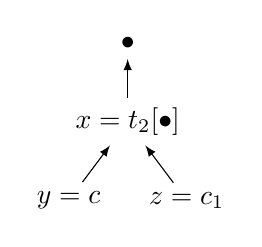
\begin{tikzpicture}[ 
  edge from parent path={(\tikzchildnode\tikzchildanchor) edge [-latex] (\tikzparentnode\tikzparentanchor)},
  level distance=1cm
]
\node (d) {$\bullet$} child{node (a) {$x=t_2[\bullet]$} child{node (b) {$y=c$}} child{node (c)
{$z=c_1$}}};

\end{tikzpicture}
\end{center}
Now each of the environments is represented by a linked list, with the binding
of $x$ shared between them. This is an example of a \emph{shared} environment
~\cite{appel1988optimizing}. This shared, linked structure dates back to the 
first machine for evaluating expressions, Landin's SECD
machine~\cite{landin1964mechanical}.

The drawbacks and advantages of each approach are well known. With a flat
environment, variable lookup can be performed with a simple offset
~\cite{jonesstg,appel1992compiling}. On the other hand, significant
duplication can occur, as I will discuss in Section~\ref{sec:exist}.
With a shared environment, that duplication is removed, but at the cost of
possible link traversal upon dereference. 

As with most topics in compilers and abstract machines, the design space is
actually more complex. For example, Appel and Jim show a wide range of hybrids
~\cite{appel1988optimizing} between the two, and Appel and Shao
~\cite{shao1994space} show an optimized hybrid that aims to achieve the benefits
of both approaches. And as shown in the next section, choice of evaluation
strategy further complicates the picture.

\section{Existing Call-by-Need Environments} \label{sec:exist}

Existing call by need machines use flat environments with a heap of
closures~\cite{jonesstg,TIM,johnsson1984efficient,boquist1997grin}. These
environments may contain some combination of primitive values and pointers into the
heap ($p$ below). The pointers and heap implement the memoization of results
required for call by need. Returning to the earlier example, $(\lambda
x.(\lambda y.t) (\lambda z.t_1)) t_2$, we can view a simplified execution state
for this approach when entering $t$ as follows:

\begin{center}
\textbf{Closure}
\begin{align*}
t[x=p_0, y=p_1] \\
\end{align*}
\textbf{Heap}
\begin{align*}
p_0 &\mapsto t_2[\bullet] \\
p_1 &\mapsto \lambda z.t_1[x=p_0] 
\end{align*}
\end{center}

Consider $t_2[\bullet]$, the closure at $p_0$. If it is not in WHNF (this sort
of unevaluated closure is called a
\emph{thunk}~\cite{ingerman1961way,peyton1992implementing}), then if it is
entered in either the evaluation of $t$ or $t_1$, the resulting value will
overwrite the closure at $p_0$. The result of the computation is then shared
with all other instances of $x$ in $t$ and $t_1$. In the case that terms have a
large number of shared variables, environment duplication can be expensive.
Compile-time transformation ~\cite{peyton1992implementing} (tupling arguments)
helps, but we show that the machine can avoid duplication completely.

Depending on $t$, either or both of the closures created for its free variables
may not be evaluated. Therefore, it is possible that the work of creating the
environment for that thunk will be wasted. This waste is well known, and
existing approaches address it by avoiding thunks as much as possible
~\cite{jonesstg,johnsson1984efficient}. Unfortunately, in cases like the above
example, thunks are necessary. I aim to minimize the cost of creating such
thunks.

Thunks are special in another way.  Recall that one advantage of flat
environments is quick variable lookups. In a lazy language, this advantage is
reduced because \emph{a thunk can only be entered once}. After it is entered, it
is overwritten with a value, so the next time that heap location is entered it
is entered with a value and a different environment. Thus, the work to ensure
that the variable lookup is fast is used for at most one evaluation of the
thunk. This is in contrast to a call-by-value language, in which every closure
is constructed for a value, and can be entered an arbitrary number of times. 

A more subtle drawback of the flat environment representation is that
environments can vary in size, and thus a value in WHNF can be too large to fit
in the space allocated for the thunk it is replacing. This problem is discussed
in~\cite{jonesstg}, where the proposed solution is to put the value closure in
a fresh location in the heap where there is sufficient room. The original
thunk location is then replaced with an indirection to the value at the freshly
allocated location. These indirections are removed during garbage collection,
but do impose some cost, both in runtime efficiency and implementation
complexity~\cite{jonesstg}.

I have thus far ignored a number of details with regard to current
implementations. For example, the STG machine can split the flat environment, so
that part is allocated on the stack and part on the heap.  The TIM allocates its
flat environments separately from its closures so that each closure is a code
pointer, environment pointer pair~\cite{TIM} while the STG machine keeps
environment and code co-located~\cite{jonesstg}. Still, the basic design
principle holds: a flat environment for each closure allows quick variable
indexing, but with an initial overhead.

To summarize, the flat environment representation in a call by need language
implies that whenever a term might be needed, the necessary environment is
constructed from the current environment.  This operation can be expensive, and
it is wasted if the variable is never dereferenced. In this work, I aim to
minimize this potentially unnecessary overhead.

Figure~\ref{fig:designspace} depicts the design space relevant to this chapter.
There are existing call by value machines with both flat and shared
environments, and call by need machines with flat environments. As far as I am
aware, I am the first to use a shared environment to implement lazy evaluation. 

It is worth noting that there has been work on lazy machines that effectively use
linked environments, which could potentially be implemented as a shared
environment, e.g., Sestoft's work on Krivine machines~\cite{sestoft}, but none
make the realization that the shared environment can be used to implement
sharing of results, which is the primary contribution of this chapter.

\begin{figure}
\begin{tabularx}{\textwidth}{l | X | X}
                & Flat Environment     & Shared Environment \\ \hline
  Call by need  & STG~\cite{jonesstg}, 
                  TIM~\cite{TIM}, 
                  GRIN~\cite{boquist1997grin} 
                & $\mathcal{\mathcal{C} \mskip -4mu \mathcal{E}}$ Machine \\
  Call by value & ZAM~\cite{leroy1990zinc}, 
                  SML/NJ~\cite{appel1991standard}
                & ZAM,
                  SECD~\cite{landin1964mechanical}, 
                  SML/NJ \\
\end{tabularx}
\caption{Evaluation strategy and environment structure design space. Each
acronym refers to an existing implementation. Some implementations use multiple
environment representations.}
\label{fig:designspace}
\end{figure}


\section{Big-Step \ce} \label{sec:cem_big}

This section reviews our big-step source semantics. A big-step semantics
has the advantage of powerful, easy-to-use induction properties. This eases
reasoning about many program properties. We will also review the small-step
semantics and prove that it implements the big-step semantics, but by showing
that our implementation preserves the big-step semantics, we prove preservation
of any inductive reasoning on the structure of evaluation tree.  

As in Chapter~\ref{chap:ce}, our source syntax is the lambda calculus with de
Bruijn indices. De Bruijn indices count the number of intermediate lambdas
between the occurrence of the variable and its binding lambda.  
\begin{align*}
 t &::= t \; t \; | \; x \; | \;  \lambda \; t \\
 x &\in \mathbb{N}
\end{align*}
The essence of the \ce semantics (Figure~\ref{fig:bigstep}) is that it
implements a shared environment, and uses its structure to share results of
computations. This makes possible a simple abstract machine that operates on the
lambda calculus directly, which is uncommon among call-by-need abstract machines
\cite{jonesstg,launchburynatural,TIM,johnsson1984efficient}. This simplifies
formalization, as we do not need to prove that intermediate transformations,
e.g., lambda lifting, are semantics-preserving. Another advantage of the \ce
machine is that it has constant-sized closures, obviating the need to reason
about re-allocating the results of computation and adding indirections required
because of closure size changes from thunk to value \cite{jonesstg}. We operate
on closures, which combine terms with pointers into the shared environment,
which is implemented as a heap. Every heap location contains a cell, which
consists of a closure and a pointer to the next environment location, which I
will refer to as the environment continuation.  Variable dereferences index into
this shared environment structure, and if/when a dereferenced location evaluates
to a value, the original closure (potentially a thunk or closure not evaluated
to WHNF) will be replaced with that value. The binding of a new variable extends
the shared environment structure with a new
cell. This occurs during application, which evaluates the left hand side to an
abstraction, then extends the environment with the argument term closed under the
environment pointer of the application. The App rule ensures that two
variables bound to the same argument closure will point to the same location in
the shared environment. Because they point to the same location by construction
of the shared environment, we can update that location with the value computed
at the first variable dereference, and then each subsequent dereference will
point to this value. The variable rule applies the update by indexing into the
shared environment structure and replacing the closure at that location with the
resulting value. It is worth noting that while the closures in the heap cells
are mutable, the shared environment structure is never mutated. This property is
crucial when reasoning about variable dereferences. The $\mu\left(l, i\right)$
function looks up a variable index in the shared environment structure by
following environment continuation pointers, returning the location and cell
pointed to by the final step. See the Coq source
for a formal treatment. Note that we require that fresh heap locations are
greater than zero. This is required for reasoning about compilation to the
instruction machine, which we will return to in Section~\ref{sec:im_semantics}.
While here we constrain fresh heap locations to be fresh with respect to the
entire heap domain, for a real implementation, this is far too strong a
constraint, as it doesn't allow any sort of heap re-use. We return to this issue
in Section~\ref{sec:discussion}, and discuss how this could be relaxed to either
allow reasoning about garbage collection or direct heap reuse.

The fact that our natural semantics is defined on the lambda calculus with de Bruijn
indices differs from most existing definitions of call-by-need, such as
Ariola's call-by-need \cite{ariola1995call} or Launchbury's lazy semantics
\cite{launchburynatural}. These semantics are defined on the lambda calculus with named
variables. While it should be possible to relate our semantics to
these, the comparison is certainly made more difficult by this
disparity.\footnote{Both of these well known existing semantics have known
problems that arise during formalization, as discussed in
Section~\ref{sec:discussion}.} A more fruitful relation to semantics operating
on the lambda calculus with named variables would likely be relating Curien's
calculus of closures to call-by-name semantics implemented with substitution. We
return to this discussion in Section~\ref{sec:discussion}.

As mentioned in Section~\ref{chap:ce}, these big-step semantics do not
explicitly include a notion of nontermination. Instead, nontermination would be
implied by the negation of the existence of an evaluation relation. This
prevents reasoning directly about nontermination in an inductive way, but for
the purpose of our primary theorem this is acceptable. 

One interesting property of defining an inductive evaluation relation in a
language such as Coq is that computation can be done on the evaluation tree. In
other words, the evaluation relation given above defines a data type, one that
computation can be done on in standard ways. For example, we could potentially
compute properties such as size and depth, which would be related to operational
properties of compiled code. 

Finally, given a term $t$, the initial configuration is defined as
$\left(t\left[0\right], \epsilon\right)$. As discussed, the choice of the null
pointer for the environment pointer is not completely arbitrary, but chosen
across our semantics uniformly to represent failed environment lookup. 

\subsection{Call-By-Name}

This section reviews the call-by-name variant of our big-step semantics and
provides a proof that it is an implementation of Curien's call-by-name calculus
of closures. 

See Figure~\ref{fig:bigstepname} for the definition of our call-by-name
semantics. Note that the only change from our call-by-need semantics is that we
do not update the heap location with the result of the dereferenced computation.
This is the essence of the difference between call-by-name and call-by-need.

Recall Figure~\ref{fig:curien} for a formalization of Curien's call-by-name
semantics. We define a heterogeneous equivalence relation between our shared
environment and Curien's environment. Effectively, this relation is the
proposition that the shared environment structure is a linked list
implementation of the environment list in Curien's semantics. This is defined
inductively, and we require that every closure reachable in the environment is
also equivalent.  We say two closures are equivalent if their terms are
identical and their environments are equivalent. 

Given these definitions, we can prove that the call-by-name \ce semantics
implements Curien's call by name semantics: 

\begin{thm}
If a closure $c$ in Curien's call-by-name semantics is equivalent to a
configuration $c'$, and $c$ steps to $v$, then there exists a $v'$ that our
call-by-name semantics steps to from $c'$ that is equivalent to $v$.
\end{thm}
\begin{proofoutline}
The proof proceeds by induction on Curien's step relation. The abstraction rule
is a trivial base case. The variable lookup rule uses a helper lemma that proves
by induction on the variable that if the two environments are equivalent and the
variable indexes to a closure, then the $\mu$ function will look up an
equivalent closure. The application rule uses a helper lemma which proves that a
fresh allocation will keep any equivalent environments equivalent, and that the
new environment defined by the fresh allocation will be equivalent to the
extended environment of Curien's semantics.
\end{proofoutline}

By proving that Curien's semantics is implemented by the call-by-name variant of
our semantics, we provide further evidence that our call-by-need is a meaningful
semantics. 

One important note is that nowhere do we require that a term being evaluated is
closed under its environment. Indeed, it's possible that a term with free variables
can be evaluated by both semantics to a value as long as a free variable is
never dereferenced. This theme will recur through the rest of the chapter, so it
is worth keeping in mind.  

\section{\ce Small-Step Semantics} \label{sec:cem_small}

In this section we discuss the small-step semantics of the \ce 
machine, and show that it implements the big-step semantics of
Section~\ref{sec:cem_big}. This is a fairly straightforward transformation implemented
by adding a stack. The source language is the same, and we simply add a stack to
our configuration (and call it a state). The stack elements are either argument
closures or update markers. Update markers are pushed onto the stack when a
variable dereferences that location in the heap. When they are popped by an
abstraction, the closure at that location is replaced by said abstraction, so
that later dereferences by the same variable in the same scope dereference the
value, and do not repeat the computation.  Argument closures are pushed onto the
stack by applications, with the same environment pointer duplicated in the
current closure and the argument closure.  Argument closures are popped off the
stack by abstractions, which allocate a fresh memory location, write the
argument closure to it, write the environment continuation as the current
environment pointer, then enter the body of the abstraction with the fresh
environment pointer. This is the mechanism used for extending the shared
environment structure. The semantics is defined formally in
Figure~\ref{fig:cesm}.  

\begin{figure}
\textbf{Syntax}
\begin{align*}
\tag{State} s &::= \langle c, \sigma, \mu \rangle \\
\tag{Term} t &::= i \; | \; \lambda t \; | \; t \; t  \\
\tag{Variable} i &\in \mathbb{N}  \\
\tag{Closure} c &::= t \left[l\right] \\
\tag{Value} v &::= \lambda t\left[l\right] \\
\tag{Heap} \mu &::= \epsilon \; | \; \mu \left[ l \mapsto \rho \right] \\
\tag{Environment} \rho &::= \bullet \; | \; c \cdot l \\
\tag{Stack} \sigma &::= \square \; | \; \sigma \; c \;  | \; \sigma \; u \\
\tag{Location} l,u,f &\in \mathbb{N}
\end{align*}
\textbf{Semantics}
\begin{align*}
\tag{Upd}
\langle v,  \sigma \; u , \mu \rangle 
  &\rightarrow
\langle v, \sigma, \mu\left(u \mapsto v \cdot l\right) \rangle  
\; \textnormal{where} \; c \cdot l = \mu\left(u\right) \\
\tag{Lam}
\langle \lambda t\left[l\right], \sigma \; c, \mu \rangle 
  &\rightarrow
\langle t\left[f\right], \sigma, \mu\left[f \mapsto c \cdot l\right]\rangle f
\not \in \textnormal{dom}\left(\mu\right)  \\
\tag{App}
\langle t \; t'\left[l\right], \sigma, \mu \rangle
  &\rightarrow
\langle t\left[l\right], \sigma \; t'\left[l\right], \mu \rangle \\
\tag{Var1}
\langle i\left[l\right], \sigma, \mu \rangle
  &\rightarrow
\langle c, \sigma \; l'', \mu \rangle
\; \textnormal{where} \; l'' \mapsto c \cdot l' = \mu\left(l, i\right)
\end{align*}
\caption{Syntax and semantics of the \ce machine}
\label{fig:cesm}
\end{figure}

Note that the presentation given here differs slightly from our previous
presentation \cite{cem}, which inlined the lookup into the machine steps. This
is to simplify formalization and relation to the big-step semantics, but does not
change the semantics of the machine. As a trade-off, it does make the relation to
the instruction machine in the later sections slightly more involved, but
it is generally a superficial change.

\subsection{Relation to Big Step}
Here we prove that the small-step semantics implements the big-step semantics of
Section~\ref{sec:cem_big}. This requires first a notion of reflexive transitive closure,
which we define in the standard way. We also make use of the fact that the
reflexive transitive closure can be defined equivalently to extend from the left
or right. 

\begin{lemma}
If the big-step semantics evaluates from one configuration to another, then the
reflexive transitive closure of the small-step semantics evaluates from the same
starting configuration with any stack to the same value configuration with that
same stack.
\end{lemma}
\begin{proofoutline}
The proof proceeds by induction on the big-step relation. We define our
induction hypothesis so that it holds for all stacks, which gives us the
desired case of the empty stack as a simple specialization. The rule for
abstractions is the trivial base case. Var rule applies as the first step, and
the induction hypothesis applies to the stack with the update marker on it. To
ensure that the Upd rule applies we use the fact that the big-step semantics
only evaluates to abstraction configurations, and the fact that the reflexive
transitive closure can be rewritten with steps on the right. For the Application
rule, we take advantage of the fact that we can append two evaluations together,
as well as extend a reflexive transitive closure from the left or the right. As
with the Var rule we use the fact that the induction rule is defined for all
stacks to ensure we evaluate the left hand side to a value with the argument on
the top of the stack.  Finally, we extend the environment with the argument
closure, and evaluate the result to a value by the second induction hypothesis.
\end{proofoutline}

Adding a stack in this fashion is a standard approach to converting between big
step and small-step semantics. Still, we appreciate that this approach applies
here in a straightforward way. 

\section{Instruction Machine} \label{sec:im_semantics}

Here we describe in full the instruction machine syntax and semantics. We choose a
simple stack machine with a Harvard architecture (with separate instruction and
heap memory). We use natural numbers for pointers, though it shouldn't be too
difficult to replace these with standard-sized machine words, e.g., 64 bits,
making the stack and malloc operations partial. Our stack is represented as a
list of pointers, though again it should be a relatively straightforward
exercise to represent the stack in contiguous memory. We define our machine to
have only four registers: an instruction pointer, an environment pointer, and
two scratch registers. Our instruction set is minimal, consisting only of a
conditional jump instruction, pop and push instructions, a move instruction, and
a new instruction for allocating new memory. Note that for our program memory, I
have pointers to basic blocks, but for simplicity of proofs we choose to not
increment the instruction pointer within a basic block.  Instead, the
instruction pointer is constant within a basic block, only changing between
basic blocks. In fact, we represent the program as a list of basic blocks, with
pointers indexing into the list. This has the advantage of letting us easily
reason about sublists and their relation to terms. The full syntax of the
machine is given in Figure~\ref{fig:im_syntax}. Note that curly brackets
$\left\{\right\}$ denote optionality, while stars $*$ denote zero or more
elements, represented as a list. Note that we'll use some common list
terminology, such as bracket notation for indexing, i.e., $l\left[i\right]$
accesses the $i$'th element in $l$ (we don't worry about the partiality in this
presentation of this operation; see the Coq implementation for a full
treatment). We also use $\concat$ for list concatenation, and $::$ for consing an
element onto the head of a list. 

\begin{figure}
\begin{align}
n, l, w &\in \mathbb{N} \tag{Machine Word} \\
r &:= ip \; | \; ep \; | \; r1 \; | \; r2 \tag{Registers} \\
wo &:= r \; | \; r \% n \tag{Write Operands} \\
ro &:= wo \; | \; n \tag{Read Operands} \\
i &:= \mathit{push} \; ro \; | \; \mathit{pop} \; wo \; | \; \mathit{new} \; n
\; wo \; | \; \mathit{mov} \; ro \; wo \tag{Instructions} \\
bb &:= i : bb \; | \; \mathit{jump} \left\{ro, l\right\} ro \tag{Basic Block} \\
p &:= bb* \tag{Program} \\
s &:= w* \tag{Stack} \\
h &:= \left(l, w\right)* \tag{Heap}\\
S &:= \langle rf, p, s, h \rangle \tag{State} 
\end{align}
\caption{Instruction Machine Syntax}
\label{fig:im_syntax}
\end{figure}

We separate read (ro) and write (wo) operands. Write operands can be registers
or memory (defined by a register and a constant offset). Read operands can be
any write operand or a constant. For reading, there is the read relation, which
takes a read operand and a state and is inhabited when the third argument can be
read from that read operand in that state. Similarly, a write relation is
inhabited when writing the second argument into the first in a state defined by
the third argument results in the state defined by the fourth argument.  

The machine semantics should be fairly unsurprising. A State, consists of a
register file, program memory, a stack, and a heap. The push instruction takes a
read operand and pushes it onto the stack. The pop instruction pops the
top of the stack into a write operand. The mov instruction moves a machine word
from a read operand to a write operand. The jump instruction is parameterized by
an optional pair, which, if present, reads the first element of the pair from a
read operand, checks if it is zero, and if so sets the IP to the second element
of the pair, which is a constant pointer. If the condition is not zero, then it
sets the IP to the instruction pointer contained in the second jump argument. If
we pass nothing as the first argument, then it becomes an unconditional set of
the IP to the value read from the second argument.  Note that the second
argument is a read operand, so it can either be a constant or read from a register
or memory. This means it can be effectively either a direct or indirect jump,
both of which are used in the compilation of lambda terms. The new instruction
allocates a contiguous block of new memory and writes the resulting pointer to
the fresh memory into a write operand. We take the approach of not choosing a
particular allocation strategy. Instead, we follow existing approaches and
parameterize our proof on the existence of such functionality
\cite{chlipala2007certified}. The complete semantics of the machine is given in
Figure~\ref{fig:im_semantics}.  Note that we separate instruction steps and
basic block steps. Recall that a basic block is a sequence of instructions that
ends with a jump. The Step BB relation will execute the instructions in the
basic block in order, then set the IP in accordance with the jump semantics. The
Step relation dereferences a basic block at the current IP, and if executing the
basic block results in a new state, then the machine executes to that state. 

\begin{figure}
\begin{gather*}
\tag{Push}
\inference{
\mathit{read} \; ro \; \langle rf, p s, h \rangle \; v \\
bb, \langle rf, p, v::s, h \rangle \rightarrow_{bb} S 
}{\mathit{push} \; ro : bb, \langle rf, p, s, h \rangle \rightarrow_{bb} S} \\ \\
\tag{Pop}
\inference{
\mathit{write} \; wo \; w \langle rf, p, s, h \rangle S' \\
bb, S' \rightarrow_{bb} S \\
}{\mathit{pop} \; wo:bb, \langle rf, p, w::s, h \rangle \rightarrow_{bb} S}  \\ \\
\tag{New} \inference{
\forall i < n, f+i \notin \textsf{dom}\left(h\right) \\
\mathit{write} \; wo \; f \langle rf, p, s, \mathit{zeroes} \; n \; f \concat h \rangle S' \\
bb, S' \rightarrow_{bb} S
}{\mathit{new} \; n \; wo:bb, \langle rf, p, s, h \rangle \rightarrow_{bb} S} \\ \\
\tag{Mov} \inference{
\mathit{read} \; ro \; s \; v \quad
\mathit{write} \; wo \; v \; S \; S' \quad
bb, S' \rightarrow_{bb} S''
}{\mathit{mov} \; ro \; wo:bb, S \rightarrow_{bb} S''} \\ \\
\tag{Jump 0} \inference{
\mathit{read} \; ro \; S \; 0 \quad
\mathit{write} \; ip \; k \; S \; S'
}{\mathit{jump} \; \left(ro, k\right) \; j, S \rightarrow_{bb} S'} \\ \\
\tag{Jump S} \inference{
l > 0 \quad 
\mathit{read} \; ro \; S \; l \\
\mathit{read} \; j \; S \; k \quad
\mathit{write} \; ip \; k \; S \; S'
}{\mathit{jump} \; \left(ro, k'\right) \; j, S \rightarrow_{bb} S'} \\ \\
\tag{Jump} \inference{
\mathit{read} \; ro \; S \; l \quad
\mathit{write} \; ip \; l \; S \; S'
}{\mathit{jump} \; ro:S \rightarrow_{bb} S'} \\ \\
\tag{Enter} \inference{
\mathit{read} \; ip \; \langle rf, p, s, h \rangle \; k \\
p\left[k\right] = bb \\
bb, \langle rf, p, s, h \rangle \rightarrow_{bb} S' 
}{\langle rf, p, s, h \rangle \rightarrow S'}
\end{gather*}
\caption{Instruction Machine Semantics}
\label{fig:im_semantics}
\end{figure}


\section{Compiler} \label{sec:compiler}

In this section I describe the compiler, which compiles lambda terms with
de Bruijn indices to programs. The compiler proceeds by recursion on lambda
terms, keeping a current index into the program to ensure correct linking
without a separate pass. For variables, when we get to zero we push the current
environment pointer and a null instruction pointer to denote the update marker
to the location of the closure being entered. Then we $\mathit{mov}$ the closure
at that location into $r1$ and $ep$, and $\mathit{jump}$ to
$r1$, recalling that the $\mathit{jump}$ sets the $ip$. For 
nonzero variables, we replicate traversing the environment pointer $i$
times before loading the closure.  For applications, we calculate the program
location of the argument basic block, and push that and the current environment
pointer onto the stack, effectively pushing an argument closure on top of the
stack. We then $\mathit{jump}$ to the left hand side of the application, as is
standard for push-enter evaluation. For abstractions, we use a conditional jump
depending on whether the top of the stack is a null pointer (and therefore an
update marker) or a valid instruction pointer (and therefore an argument). If it
is an update marker, we update the heap location defined by the update marker
with the current value instruction pointer and the current environment pointer.
We must point to the first of the three abstractions basic blocks, as this value
could later update another heap location as well. In the case that the top of
the stack was a valid instruction pointer, we allocate a new chunk of 3 word of
memory, and $\mathit{mov}$ the argument closure into it, with the current
environment pointer as the environment continuation. We then set our current
environment pointer to this fresh location. This is the process by which we
extend our shared environment structure in the instruction machine. Finally, we
perform an unconditional jump to the next basic block, which is the first basic
block of the compiled body of the lambda. As this is an unconditional jump to
the next basic block, for real machine code this jump can be omitted. 

\begin{figure}
\begin{align*}
\mathit{var} \; 0 :=  \;
  &\mathit{push} \; ep : \\
  &\mathit{push} \; 0 : \\
  &\mathit{mov} \; \left(ep\%0\right) \; r1 : \\
  &\mathit{mov} \; \left(ep\%1\right) \; ep : \\
  &\mathit{jump} \; r1 \\
\mathit{var} \; \left(i+1\right) := \;
  &\mathit{mov} \; \left(ep\%2\right) \; ep : \\
  &\mathit{var} \; i \\
\mathit{compile} \; i \; k := \; & \left[\mathit{var} \; i\right] \\
\mathit{compile} \; \left( m \; n \right) \; k := \;
  &\mathit{let} \; ms = \mathit{compile} \; m \; \left(k+1\right) \; in \\
  &\mathit{let} \; nk = 1+k+length \; ms \; in \\
  &\mathit{push} \; ep :  \\
  &\mathit{push} \; nk : \\
  &\mathit{jump} \; \left(k+1\right) :: \\
  &ms \concat \mathit{compile} \; n \; nk \\
\mathit{compile} \; \left(\lambda b\right) \; k := \;
  &\mathit{pop} \; r1 : \\
  &\mathit{jump} \; \left(r1, k+1 \right) \; \left(k+2\right) :: \\
  &\mathit{pop} \; r1 : \\
  &\mathit{mov} \; k \; r1\%0 : \\
  &\mathit{mov} \; ep \; r1\%1 : \\
  &\mathit{jump} \; k :: \\
  &\mathit{new} \; 3 \; r2 : \\
  &\mathit{mov} \; r1 \; \left(r2\%0\right) : \\
  &\mathit{pop} \; \left(r2\%1\right) : \\
  &\mathit{mov} \; ep \; \left(r2\%2\right) : \\
  &\mathit{mov} \; r2 \; ep : \\
  &\mathit{jump} \; \left(k+3\right) :: \\
  &\mathit{compile} \; b \; \left(k+3\right)
\end{align*}
\caption{Compiler Definition}
\label{fig:compiler}
\end{figure}

Being able to define the full compiler this simply is crucial to this
verification project. Other, more sophisticated implementations of call-by-need,
such as the STG machine, are much harder to implement and reason about. It is
worth noting that despite this simplicity, initial tests suggest that performance
is not as horrible as one might suspect, and is often competitive with state of
the art \cite{cem}.

As with the relation discussed in Section~\ref{sec:cem_big}, a term does not
have to be closed to compile it. Indeed, we will happily generate code that if
entered, will attempt to dereference the null pointer, leaving the machine
stuck. Because I am only concerned with proving that the source semantics are
implemented in the case that it evaluates to a value, this is not a problem. If
I wanted to strengthen our proof further, I would try to show that if the source
semantics gets stuck trying to dereference a free variable, the implementation
would get stuck in the same way, both failing to dereference a null pointer.    

\section{Compiler Correctness} \label{sec:correctness}

In this section we define a relation between the state of the small-step
semantics and the state of the instruction machine semantics, and show that the
instruction machine implements the small-step semantics under that relation. 

In general, we implement closures as instruction pointer, environment pointer
pairs. For the instruction pointers, we relate them to terms via the compile
function defined in Section~\ref{sec:compiler}. Essentially, we require that the
instruction pointer points to a list of basic blocks that the related term
compiles to. For the current closure, we relate the instruction pointer register
in the instruction machine to the current term in the small-step source
semantics. The environment pointers of each machine are more similar. Given a
relation between the heaps of the two machines, we define the relation between
two environment pointers as existing in the relation of the heaps, or both being
the null pointers. While it should be possible to avoid this special case,
during the proof it became apparent that not having the special case made the
proof significantly harder. This forces us to add the constraint to all machines
that pointers are non-null, which for real hardware shouldn't be an issue.  

We use null pointers in two crucial ways. One is to explicitly define the root
of the shared environment structure in both the source semantics and the machine
semantics. The other use is for instruction pointers. To differentiate between update
markers and pointers to basic blocks, we use a null pointer to refer to an
update marker, and a non-null pointer as an
instruction pointer for an argument closure. Note that in fact, while the null
pointers in heaps required us to only allocate non-null fresh locations in the
heaps of our semantics, using null pointers to denote update markers requires no
change to our program generation, due to the fact that an argument term of an
application cannot occur at position 0 in the program.

The relation between the heaps of the small-step source semantics and the
instruction machine is the trickiest part of the state relation. Note that for
each location in the source semantics heap, we have a cell with a closure and
environment continuation pointer. Naturally, the instruction machine represents
these as three pointers: two for the closure (the instruction pointer and
environment pointer) and one for the environment continuation. The easiest
approach turned out to be to use the structure of the heap constructs to define a
one-to-three mapping between this single cell and the three machine words. The
structure used for each of the heaps is a list of pointer, value bindings.
We use the ordering of these bindings in the list to define a one binding to
three binding mapping between the source heap and the machine heap. We define 
a membership relation that defines when an element is in our heap relation,
proceeding recursively on the inductive relation structure. This allows us to
define a notion of which pairs of each type of closure are in the heap, along
with their respective locations. Due to the ordering in which they are allocated
in the heap during evaluation, each pair of memory allocations corresponds to an
equivalent cell. We use this property as a heap equivalence property that is
preserved through evaluation: every binding pair in the heap relation property
described above defines equivalent closures and environment continuations. For
the relation between our stacks, we define a similar notion.  For update
markers, we require that every update marker points to related environments
(they are two pointers that exist in the heap relation). For argument closures,
we require that the closures are equivalent (the instruction pointer and
environment pointer are equivalent to their respective counterparts in the
small-step semantics). 

In summary, we require that the current closure in the small-step semantics is
equivalent to the closure represented by the instruction pointer, environment
pointer pair, and that the stacks and the heaps are equivalent. The actual Coq
implementation of this relation is too involved to relate directly here. We
encourage the reader to read the linked Coq source to fully appreciate it.

Given this relation between heaps, we can state our primary lemma.
\begin{lemma} \label{lem:cesm_im}
Given that an instruction machine state $i$ is related to a small-step
semantics state $s$, and that small-step semantics state steps to a new state
$s'$, the instruction machine will step in zero or more steps to a related state
$i'$.
\end{lemma}
\begin{proofoutline}
Our proof proceeds by case analysis on the step rules for the small-step
semantics. We'll focus on the second half of the proof, that $i'$ is related to
$s'$. The proofs that $i$ evaluates to $i'$ follow fairly directly from the
compiler definition given in Section~\ref{sec:compiler}. For the Var rule,
because we need to proceed by induction, we have to define a separate lemma and
proceed by induction on a basic block while forgetting the program, as the
induction hypothesis is invalid in the presence of the program. We then use the
lemma to show that evaluation of a compiled variable implements the evaluation
of the variable in the small-step semantics. In particular, we use the null
environment as a base case for our induction, as we know the only way lookup
could fail is if both environment pointers are null, but that cannot be the
case due to the fact that we know that the small-step semantics must have
successfully looked up its environment pointer in the heap. Therefore the only
option is for both environment pointers to exist in the heap relation, which
when combined with the heap equivalence relation in the outer proof gives us the
necessary property that the environment continuations are equivalent. Finally,
because the last locations reached must have been in the heap relation, we know
they are equivalent environment pointers, and therefore the stack relation is
preserved when we push the update marker onto the heap. For the App rule, we use
the definition of our compiler to prove that the argument term and argument
instruction pointer are equivalent and that the left hand side term and
instruction pointer are also equivalent. They share an environment pointer which
is equivalent by the fact that the application closures are related.  This
proves that the stack relation is preserved as well as the current closure,
while the heap is unchanged. For the Lam rule, we allocate a fresh variable and
because of our stack relation we can be sure that the closures that we
allocate are equivalent, as well as the environment continuations, as they are
taken from the previous current continuation. Because of how we define it, the
new allocations are equivalent under our heap relation, and preserve heap
equivalence. Finally, the Upd rule trivially preserves the stack and current
closure relations, and for proving that the relation is preserved for the
heap, we proceed by induction on the heap relation. In addition, we must prove
a supporting lemma that all environment relations are preserved by the update.
\end{proofoutline}

We now have a proof that the small-step semantics implements the big-step
semantics, and a proof that the instruction machine implements the small-step
semantics. We can now combine these to get our correct compiler theorem. 

\begin{thm} 
\label{thm:correctness}
If a term $t$ placed into the initial configuration for the big-step semantics
evaluates to a value configuration $v$, then the instruction machine starting
in the initial state with \texttt{compile 0 t} as its program will evaluate to a
related state $v'$.  
\end{thm}
\begin{proofoutline}
We first require that the relation defined between the small-step semantics
state and the instruction machine state holds for the initial configurations.
This follows fairly directly from the definition of the initial conditions and
the compile function. Second, we have by definition of reflexive transitive
closure that Lemma~\ref{lem:cesm_im} implies that if the reflexive transitive
closure of the small-step relation evaluates in zero or more steps from a
state $c$ to a state $v$, then a related state of the instruction machine $c'$
will evaluate to a state $v'$ which is related to $v$. We use these two facts,
along with the proof that the small-step implements the big-step for any stack,
specialized on the empty stack, to prove our theorem. 
\end{proofoutline}

It is worth recalling exactly what the relation implies about the two value
states. Namely, in addition to the value closures being equivalent, their heaps
and environments are equivalent, so that every reachable closure in the
environment is equivalent between the two.



\section{Discussion} \label{sec:discussion}

Here we reflect on what we have accomplished, including threats to validity,
future work, related work, and general discussion of the results.

One thing we'd like to communicate is the difficulty we had in writing
comprehensible proofs. The reader is discouraged from attempting to understand
the proofs in any way by reading the Coq tactic source code. While we attempted
to keep our definitions and lemmas as clean and comprehensible as possible, we
found it extremely difficult to do the same with tactics. Partially this may be
a failure on our part to become more familiar with the tactic language of Coq,
but we suspect that the imperative nature of tactic proofs prevents
composability of tactic meta-programs. 

Another lesson was the importance of good induction principles. For example, in
Section~\ref{sec:threats}, we will discuss the issue of only proving the
implication of correctness in one direction. This is effectively a product of
the power of the inductive properties of high level semantics, which makes them
so much easier to reason about. Indeed, this lesson resonates with the purpose
of the chapter, which is that we'd like to reason about high level semantics,
because they are so much easier to reason about due to their pleasant inductive
properties, and have that reasoning preserved through compilation. 

\subsection{Threats to Validity} \label{sec:threats}

There are a few potential threats to validity that we address in this section. The
first is the one mentioned in Section~\ref{sec:background}, that we only show
that our compiler is correct in the case of termination of the source semantics.
In other words, if the source semantics doesn't terminate, we can say nothing
about how the compiled code behaves. This means that we could have a compiled
program that terminates when the source semantics does not terminate.

One argument in defense of our verification is that \emph{we generally only care
about preservation of semantics for preserving reasoning about our programs}. In
other words, if we have a program that we can't reason about, and therefore may
not terminate, we care less about having a proof that semantics are preserved.
Of course, this is a claim about most uses of program analysis. There are
possible analyses that could say things along the lines of \emph{if} the source
program terminates, then we can conclude $x$. We claim these cases are rare, and
therefore the provided proof of correctness can still be applied to most use
cases.  

Another potential threat to validity is the use of a high level instruction
machine language. While we claim that its high level and simplicity should make
it possible to show that a set of real ISAs implement this instruction machine,
we haven't formally verified this step. We believe that this would make
for valuable future work, and hope that the reader agrees that nothing in the
design of our high level instruction machine would prevent such work.

As a dual to the issue of a high level instruction machine language, some
readers may take issue with calling lambda calculus with de Bruijn indices an
"input language". Indeed, we do not advocate writing programs in such a
language. Still, the conversion between lambda calculus with named variables and
lambda calculus with de Bruijn indices is a well understood topic, and we
believe it would distract from the presentation of the verified compiler
provided here. Indeed, as noted below, semantics using named variables and
substitution can be hard to get right \cite{breitnerthesis, nakata2009small}, so
we stand by our decision to use a semantics based on lambda calculus with de
Bruijn indices. One potential approach for future work would be to prove that a
call-by-name semantics using substitution is equivalent to Curien's calculus of
closures, which when combined with a proof that our call-by-need implements our
call-by-name, would prove the compiler implements the semantics of a standard
lambda calculus with named variables.

A third threat to the validity of this work is the question of whether 
we have really proved that we have implemented \emph{call-by-need}. The question
naturally arises of what exactly it means to prove an implementation of
call-by-need is correct. There are certainly well-established semantics
\cite{launchburynatural, ariola1995call}, so one option would be to directly
prove that the $\mathcal{CE}$ semantics implements one of those existing
semantics.  Unfortunately, recent work has shown that both of these have small
issues that arise when formalized that require fixes. Indeed, we did stray down
this path a good ways and discovered one of these issues which has been
previously described in the literature \cite{nakata2009small}. This raises the
question of whether or not semantics that aren't obviously correct are a good
base for what it means to be a call-by-need semantics. Instead, we have chosen to
relate our call-by-name semantics formally to a semantics that is obviously
correct, Curien's calculus of closures. Along with the small modification
required for memoization of results, we hope that we have convinced the reader
that it is \emph{extremely likely} that the memoization of results is correct.
Of course, further evidence such as examples of correct evaluation would go
further to convince the reader, and for that we encourage readers to
play with a toy implementation at \url{https://github.com/stelleg/cem_pearl}.
Finally, a more convincing result would be a proof that the call-by-need
semantics implement the call-by-name semantics. 

Yet another threat to validity is our approach (or lack of approach) to
heap-reuse. For simplicity, we have assumed that our fresh locations are fresh
with respect to all existing bindings in the heap. Of course, this is
unsatisfactory when compared to real implementations. It would be preferable to
have our freshness constraint relaxed to only be fresh with respect to live
bindings on the heap. We believe that this modification should be possible, at
the cost of increased complexity in the proofs. 

\subsection{Future Work}

In addition to some of the future work discussed as ways of addressing issues 
in Section~\ref{sec:threats}, there are some additional features that we think
make for exciting areas of future work. 

One such area is reasoning about preservation of operational properties such as
time and space requirements. This would enable reasoning about time and space
properties at the source level and ensuring that these are preserved through
compilation. In addition, there is the possibility of verified optimizations,
where one can prove that some optimizations are both \emph{correct}, in that
they provably preserve semantics, and \emph{true} optimizations, in that they
only improve performance with respect to some performance model. By defining a
baseline compiler and proving that it preserved operational properties such as
time and space usage, one would have a good platform for which to apply this
class of optimizations, resulting in a full compiler that verifiably preserves 
bounds on time and space consumption. As with correctness, reasoning about
operational properties is often likely to be easier in the context of the
easy-to-reason-about high level semantics, and having that reasoning provably
preserved would be extremely valuable. 

Another exciting area of future work is powerful proofs of type preservation
through compilation.  While there has been existing work on type-preserving
compilers, fully verified compilers like this one provide such a strong property
that type-safety should fall out directly.

One useful feature of Coq is the ability to extract Coq programs out to other
implementations, e.g. Haskell. This raises the possibility of extracting the
verified compiler out to a Haskell implementation that could be incorporated
into GHC, providing a path towards a verified Haskell compiler. 

\subsection{Relation to Ariola et al.}

As mentioned above, to improve the relation to existing work, we could relate
the semantics to the operational semantics of Ariola et al., seen in
Figure~\ref{fig:cbn} ~\cite{ariola1995call}. Because I spent a large amount of
time attempting this, we use this section to discuss challenges to this
approach. 

One approach I tried was to show bisimulation between $\rightarrow_{N}$ and
$\Downarrow$. Unfortunately, as mentioned in Section~\ref{sec:threats}, there is
an issue I discovered when formalizing this semantics. Essentially, the rules
for variable freshness are insufficient. To fix this, one has to modify the
rules to ensure global freshness. This modification is shown in
Figure~\ref{fig:cbn_fixed}. While it makes the semantics more complicated, the
real challenge for proving bisimulation comes from the complexity of managing  

\begin{figure}
\begin{align*}
\tag{Heap} \Phi, \Psi, \Upsilon &::= x_1 \mapsto t_1, \dots, x_n \mapsto t_n
\end{align*}
\begin{align*}
\tag{Id} \inference
{\langle \Phi \rangle t \Downarrow \langle \Psi \rangle \lambda x.t'}
{\langle \Phi, x \mapsto t, \Upsilon \rangle x \Downarrow \langle \Psi, x
\mapsto \lambda x.t', \Upsilon \rangle \lambda x.t'}
\end{align*}
\begin{align*}
\tag{Abs} \inference 
{}
{\langle \Phi \rangle \lambda x . t \Downarrow \langle \Phi \rangle \lambda x.t}
\end{align*}
\begin{align*}
\tag{App} \inference
{\langle \Phi \rangle t_l \Downarrow \langle \Psi \rangle \lambda 
x.t_n \\ \langle \Psi, x' \mapsto t_m \rangle [x'/x]t_n \Downarrow \langle
\Upsilon \rangle \lambda y.t'}
{\langle \Phi \rangle t_l \; t_m \Downarrow \langle \Upsilon \rangle \lambda y.t'}
\end{align*}
\caption{Ariola et. al's Operational Semantics}
\label{fig:cbn}
\end{figure}

By retaining the whole heap, we ensure global freshness of new variables. 

\begin{figure}
\begin{align*}
\tag{Heap} \Phi, \Psi, \Upsilon &::= x_1 \mapsto t_1, \dots, x_n \mapsto t_n
\end{align*}
\begin{align*}
\tag{Id} \inference
{\langle \Phi, x \mapsto t, \Upsilon \rangle t \Downarrow \langle \Phi', x \mapsto t, \Upsilon' \rangle \lambda x.t'}
{\langle \Phi, x \mapsto t, \Upsilon \rangle x \Downarrow 
 \langle \Phi', x \mapsto \lambda x.t', \Upsilon' \rangle \lambda x.t'}
\end{align*}
\begin{align*}
\tag{Abs} \inference 
{}
{\langle \Phi \rangle \lambda x . t \Downarrow \langle \Phi \rangle \lambda x.t}
\end{align*}
\begin{align*}
\tag{App} \inference
{\langle \Phi \rangle t_l \Downarrow \langle \Psi \rangle \lambda 
x.t_n \\ \langle \Psi, x' \mapsto t_m \rangle [x'/x]t_n \Downarrow \langle
\Upsilon \rangle \lambda y.t'}
{\langle \Phi \rangle t_l \; t_m \Downarrow \langle \Upsilon \rangle \lambda y.t'}
\end{align*}
\caption{Ariola et. al's Operational Semantics (Fixed)}
\label{fig:cbn_fixed}
\end{figure}

\subsection{Related Work}

Chlipala implements a compiler from a STLC to a simple instruction machine in
\cite{chlipala2007certified}. In many ways it is more sophisticated than our 
work: it converts to CPS, performs closure conversion, and proves a similar
compiler correctness theorem to the one we've proved here. The primary
difference is that we've defined a call-by-need compiler, which forces us to
reason about updating thunks in the heap, a challenge not faced by
call-by-value implementations.

Breitner formalizes Launchbury's natural semantics and proves an optimization is
sound with respect to the semantics \cite{launchburynatural,breitnerthesis}. By
relating his formalization with ours, these projects could be combined to prove
a more sophisticated lazy compiler correct: one with non-trivial optimizations
applied.

CakeML \cite{cakeml14} is a verified compiler for a large subset of the Standard
ML language formalized in HOL4 \cite{slind2008brief}. Like Chlipala's work, this
is a call-by-value language, though they prove correctness down to an x86
machine model, and are working with a much larger real-world source language.
They also make divergence arguments along the lines of \cite{functionalbigstep},
strengthening their correctness theorem in the presence of nontermination. It's
also worth noting that like \cite{leroy2012compcert}, they are also formalizing
a front end to the compiler. 

As part of the DeepSpec project, Weirich et al. have been working on formalizing
Haskell's core semantics \cite{weirich2017spec, spector2018total}. We believe
there is opportunity to use this effort in combination with the DeepSpec project
to implement and verify a full-featured Haskell compiler.


\section{Conclusion} \label{sec:conc}

Lazy evaluation has long suffered from high overhead when delaying computations.
While strictness analysis helps to alleviate this issue, there are and there
always will be cases it cannot catch. Existing implementations choose to pay an
up-front cost of constructing a flat environment to ensure efficient variable
lookup if a delayed computation is used. When a delayed computation is never
used, this overhead is wasted. In this chapter we have presented a novel approach
that minimizes this overhead. We have achieved this overhead minimization by
taking an old idea, shared environments, and using them in a novel way. By
leveraging the structure inherent in a shared environment to share results of
computation, we have avoided some of the overheads involved in delaying a
computation. 

We conclude by summarizing the key points of this chapter. First, a shared
environment, explicitly represented as a cactus stack, is a natural way to share
the results of computation as required by lazy evaluation. Second, this approach
is in a sense \emph{lazier} about lazy evaluation than existing implementations
because it avoids some unnecessary packaging. Third, this approach can be
formalized in both big-step and small-step semantics. Lastly, the abstract
machine can be implemented as a compiler in a straightforward way, yielding
performance comparable to existing implementations. 


% We recommend abbrvnat bibliography style.
\bibliographystyle{abbrvnat}
\bibliography{annotated}

\end{document}
